%----------------------------------------------------------------------------------------------------------------------------
\graphicspath{{Parti/P04-Travi_rigide/C03-Assemblaggi_travi/Figure/}}
\chapter{Assemblaggi di travi: tipologie}
\label{cap:assemblaggi_travi}
%----------------------------------------------------------------------------------------------------------------------------

\begin{sommario}
	Si estende l'analisi della trave singola ai sistemi
	di travi piane, mostrando come la teoria dei sistemi
	di corpi rigidi sviluppata nei
	\CAPref{cap:problemi_cin_stat_SCR},
	\ref{cap:classificazione_sol_SCR}
	e~\ref{cap:classificazione_SCR}
	si trasferisca senza modifiche al contesto delle travi.
	Si classificano le connessioni tra travi in base alle
	componenti di spostamento che vincolano e alle
	caratteristiche della sollecitazione che trasmettono,
	ricavando per ciascuna tipologia la \emph{molteplicità}
	$m_i$ del collegamento, e si presenta la procedura
	operativa per l'impostazione dell'analisi.
	
	Si costruisce quindi un catalogo delle principali
	tipologie strutturali, organizzato secondo la natura
	delle connessioni, con rinvio ai capitoli dedicati.
	I \emph{sistemi a connessioni eterogenee} e i
	\emph{sistemi reticolari} sono trattati nel
	Vol.~I perché ammettono configurazioni isostatiche
	analizzabili con il solo equilibrio. Per i sistemi
	a \emph{connessioni omogenee} si introduce la
	\emph{doppia lettura topologica}, in cui i nodi
	diventano i protagonisti e le travi i vincoli.
	Le configurazioni iperstatiche di tutte le tipologie
	--- e i \emph{telai} nella loro interezza ---
	richiedono il legame costitutivo tra sforzi e
	deformazioni, sviluppato nel Vol.~II.
\end{sommario}


%----------------------------------------------------------------------------------------------------------------------------
\section{Travi e sistemi di travi: raccordo con la teoria
	dei SCR}
\label{sec:raccordo_SCR}
%----------------------------------------------------------------------------------------------------------------------------

Nei capitoli precedenti della Parte~III sono stati sviluppati
il modello della trave singola~(\CAPref{cap:Trave_Rigida}) e
i metodi per il calcolo delle caratteristiche della
sollecitazione su di essa~(\CAPref{cap:Diagrammi_CS}).
Per passare agli \emph{assemblaggi di travi}\index{assemblaggio di travi|textbf} --- strutture
composte da più travi collegate tra loro e vincolate al suolo
--- non è necessaria alcuna teoria aggiuntiva: la struttura
matematica che governa questi sistemi è già stata costruita
interamente nella Parte~II, dove si è trattata la meccanica
dei sistemi di corpi rigidi~(SCR).

Il presente capitolo ha perciò un compito preciso: mostrare
come la trave, nella sua veste di corpo rigido con caratteristiche
intrinseche, si inserisca nella cornice dei SCR,
e costruire il \emph{catalogo} delle tipologie strutturali
più importanti che emergono dalla combinazione di travi e
connessioni di diversa natura.


%............................................................................................................................
\subsection{La trave come corpo rigido piano}
\label{subsec:trave_SCR}
%............................................................................................................................

Dal punto di vista della \emph{cinematica infinitesima},
una trave piana è un corpo rigido la cui geometria è
caratterizzata da una dimensione predominante, la lunghezza.
La sua configurazione è pertanto descritta, nel caso piano,
da tre parametri cinematici: due componenti di traslazione
e una rotazione, raccolti --- scelto un polo di riduzione
$O$ --- nel vettore
\begin{equation}
	\bm{u}_e
	=
	\bigl(
	u(O)\,\; v(O)\,\; \vartheta
	\bigr)^{\!\top}
	\in \mathbb{R}^{3},
\end{equation}
del tutto analogo al vettore di configurazione del singolo
corpo rigido del \CAPref{cap:problemi_cin_stat_SCR}.

Per un sistema di $n_e$ travi\index{sistema di travi}, il vettore di configurazione
globale ha dimensione $n = 3n_e$\nomenclature[L]{$n_e$}{numero di travi (elementi) del sistema} e si costruisce
concatenando i vettori dei singoli elementi, esattamente
come nella \EQUref{eq:vettore_u} per i sistemi di corpi
rigidi generali. La formula fondamentale di classificazione
\begin{equation}\label{eq:class_travi}
	g_\ell - g_{\mathscr{i}} = \nu, \qquad
	\nu \coloneqq 3n_e - m,
\end{equation}
dove $m$ è il numero complessivo di equazioni scalari di
vincolo (molteplicità totale dei vincoli), si applica
immediatamente, con la sola sostituzione $n_c \to n_e$.

\begin{oss}
	La formula~\eqref{eq:class_travi} non dipende dal
	modello di deformabilità adottato per le travi: essa è
	una proprietà della \emph{topologia} del sistema
	(numero di travi, numero e tipo di vincoli) e non
	delle proprietà meccaniche degli elementi. Questo è
	coerente con il fatto che la classificazione isostatica
	--- o isodeterminata --- è un concetto cinematico e
	statico, non costitutivo.
\end{oss}


%............................................................................................................................
\subsection{Comportamento esterno e comportamento interno}
\label{subsec:est_int}
%............................................................................................................................

Nei sistemi di travi è utile distinguere due livelli di
comportamento cinematico, che possono dare luogo a
classificazioni diverse.

Il \emph{comportamento esterno}\index{comportamento esterno|textbf} riguarda i movimenti
rigidi del sistema nel suo insieme rispetto all'ambiente.
Esso dipende esclusivamente dai vincoli che collegano
il sistema al suolo (vincoli esterni) e si analizza
trattando il sistema come se fosse un unico corpo rigido.
Un sistema è \emph{isostatico esternamente}\index{isostaticita@isostaticità!esterna} se i vincoli
al suolo sono in numero e disposizione tali da impedire
qualsiasi moto rigido d'insieme: esso non è né labile
né iperstatico dal punto di vista esterno.

Il \emph{comportamento interno}\index{comportamento interno|textbf} riguarda invece i movimenti
relativi tra le travi del sistema, indipendentemente dai
vincoli al suolo. Esso dipende dalla topologia delle
connessioni interne. Un sistema può avere meccanismi interni
(labilità interna) anche se è bloccato al suolo in modo
isostatico; viceversa, può presentare iperstaticità interna
senza che i vincoli al suolo siano sovrabbondanti.


La separazione tra comportamento esterno e interno ha
conseguenze pratiche rilevanti: consente di affrontare
l'analisi in due fasi distinte, identificando dapprima
la classificazione del sistema nel suo insieme rispetto
al suolo, e poi quella delle relazioni cinematico-statiche
tra le travi. Questa procedura a due livelli sarà applicata
sistematicamente nel catalogo del \PARref{sec:catalogo}.


\begin{oss}
	La distinzione esterno/interno è duale: la
	\emph{labilità interna}\index{labilita@labilità!interna} corrisponde, sul versante
	statico, a stati di sollecitazione interni che si
	auto-equilibrano senza reazioni al suolo; la
	\emph{iperstaticità interna}\index{iperstaticita@iperstaticità!interna} corrisponde a condizioni
	di compatibilità cinematica che devono essere soddisfatte
	dalle distorsioni e dai cedimenti interni. Questa
	dualità è una manifestazione della struttura
	$\bm{B} = \bm{A}^{\top}$ che governa l'intero volume.
\end{oss}

%............................................................................................................................
\subsection{La molteplicità dei vincoli nei sistemi di travi}
\label{subsec:molt_travi}
%............................................................................................................................

Nella formula~\eqref{eq:class_travi}, il numero $m$ di
equazioni scalari di vincolo\index{vincolo!molteplicità} si calcola come somma
di due contributi:
\begin{equation}\label{eq:m_travi}
	m = m_{\text{est}} + m_{\text{int}},
\end{equation}
dove $m_{\text{est}}$\nomenclature[L]{$m_{\text{est}},\,m_{\text{int}}$}{molteplicità complessiva dei vincoli esterni e interni} è la molteplicità complessiva dei
vincoli esterni (tra travi e suolo) e $m_{\text{int}}$ è la
molteplicità complessiva dei vincoli interni (tra travi
diverse).

Le molteplicità dei vincoli esterni sono quelle già
tabulate nel \CAPref{cap:vincoli_CR}: il carrello contribuisce
con $m = 1$, la cerniera con $m = 2$, l'incastro con
$m = 3$. La tipologia e la molteplicità dei vincoli interni
sono invece il tema della \SECref{sec:connessioni} che segue,
dove si mostra come la natura della connessione tra travi
determini sia il numero di equazioni cinematiche di vincolo
sia le caratteristiche della sollecitazione trasmesse.

\begin{oss}
	Il calcolo di $m_{\text{int}}$ per i sistemi di travi
	richiede di identificare correttamente il tipo di
	connessione in ogni nodo interno e il numero $e_i$
	di travi che vi convergono. La molteplicità del nodo
	non è la somma delle molteplicità delle singole
	connessioni a coppie, ma dipende dalla struttura
	delle relazioni di congruenza tra tutti gli elementi
	convergenti: si veda la \EQUref{eq:molt_nodo} nella
	\SECref{sec:connessioni}.
\end{oss}


%----------------------------------------------------------------------------------------------------------------------------
\section{Connessioni tra travi: tipologie e molteplicità}
\label{sec:connessioni}
%----------------------------------------------------------------------------------------------------------------------------

La natura delle connessioni\index{connessione|textbf} tra le travi di un sistema è il
primo dato strutturale da identificare: essa determina
contemporaneamente quante equazioni cinematiche di vincolo
entrano nella formula~\EQUref{eq:class_travi} e quali
caratteristiche della sollecitazione vengono trasmesse
da una trave all'altra. Ogni tipo di connessione ammette
pertanto una doppia lettura --- cinematica e statica ---
che sono l'espressione della dualità $\bm{B} = \bm{A}^{\top}$
nel contesto dei sistemi di travi.

Le condizioni di congruenza cinematica al nodo sono
espresse nel riferimento globale $(x, y)$, dove ha senso
imporre l'uguaglianza degli spostamenti di travi con
orientamenti diversi. Le caratteristiche della
sollecitazione trasmesse sono invece grandezze locali,
riferite al sistema intrinseco di ciascuna trave; il
raccordo tra i due sistemi di riferimento è parte del
metodo dei corpi liberi (\CAPref{cap:classificazione_sol_SCR}).

Nei paragrafi che seguono si esaminano le tre tipologie
fondamentali --- nodo rigido, cerniera interna, carrello
interno --- e si ricava per ciascuna la molteplicità
$m_i$ del collegamento e le caratteristiche trasmesse.
Si introduce infine la formula generale valida per nodi
in cui convergono $e_i$ travi.


%............................................................................................................................
\subsection{Nodo rigido}
\label{subsec:nodo_rigido}
%............................................................................................................................

Il \emph{nodo rigido}\index{nodo!rigido|textbf} è la connessione più vincolante:
gli elementi che vi convergono condividono integralmente
spostamenti e rotazione nel punto di connessione. Nel caso
piano, le condizioni di congruenza tra due travi $e$ ed
$e'$ che si incontrano rigidamente nel nodo $i$ sono:
\begin{equation}\label{eq:cong_nodo_rigido}
	u_e(i) = u_i, \quad
	v_e(i) = v_i, \quad
	\vartheta_e(i) = \vartheta_i, \qquad \forall\, e \in \mathcal{E}_i,
\end{equation}
dove $(u_i, v_i, \vartheta_i)$ sono le componenti dello
spostamento nodale globale nel nodo $i$, condivise da
tutte le travi convergenti, $\mathcal{E}_i$ è l'insieme
dei loro indici e $e_i = |\mathcal{E}_i|$\nomenclature[L]{$e_i$}{numero di travi convergenti nel nodo $i$} è il loro numero.


\paragraph{Lettura cinematica.}
Il nodo rigido impone la \emph{continuità completa}
di tutti e tre i gradi di libertà cinematici nel nodo.
La sua molteplicità tra due travi è pertanto $m_i = 3$\nomenclature[L]{$m_i$}{molteplicità della connessione interna $i$}:
contribuisce con tre equazioni alla matrice dei vincoli~$\bm{A}$.

\paragraph{Lettura statica.}
Il nodo rigido trasmette integralmente \emph{tutte le
	caratteristiche della sollecitazione}: forza normale $N$,
taglio $T$ e momento flettente $M$.
Le equazioni di equilibrio al nodo esprimono la continuità
degli sforzi tra gli elementi convergenti: le sollecitazioni
di estremità di un elemento si equilibrano con quelle degli
altri elementi e con gli eventuali carichi concentrati nel
nodo. Le sollecitazioni di estremità di ciascun elemento si bilanciano
con quelle degli altri e con gli eventuali carichi concentrati nel
nodo, in tre equazioni scalari --- tante quante le caratteristiche
trasmesse, e quante i gradi di libertà condivisi.

In questa e nelle tipologie di connessione che seguono,
le caratteristiche della sollecitazione sono riferite al
sistema locale di ciascuna trave. Quando le travi
convergenti non sono ortogonali, la reazione interna
va decomposta nelle componenti di ciascun sistema locale:
questa operazione fa parte del metodo dei corpi liberi
e sarà illustrata negli esempi del \CAPref{cap:sistemi_conn_eterogenee}.


La \FIGref{fig:nodo_rigido} illustra la convenzione
grafica e le grandezze coinvolte.


%%%%%%%%%%%%%%%%%%%%%%%%%%%%%%%%%%%%%%%%%%%
\begin{figure}[htbp]
	\centering
	\resizebox{0.8\textwidth}{!}{%
		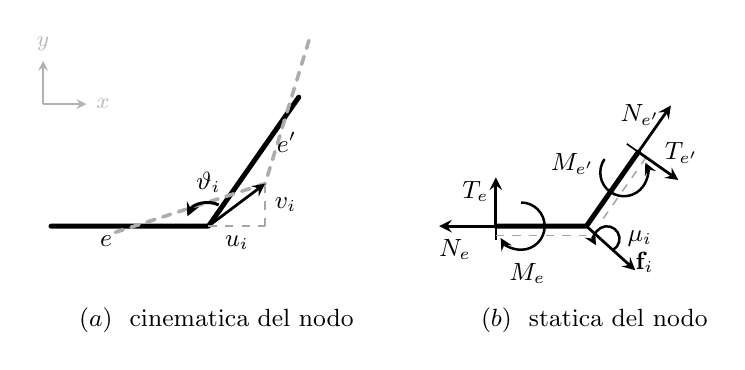
\begin{tikzpicture}[
			trave/.style={line width=1.8pt, line cap=round, line join=round, black},
			ghost/.style={line width=1.3pt, dashed, line cap=round, line join=round, gray!65},
			forza/.style={->, >=stealth, line width=1.0pt, black},
			momento/.style={->, >=stealth, line width=0.9pt, black},
			guida/.style={line width=0.55pt, dashed, gray!70},
			taglio/.style={line width=0.6pt, black},
			asse/.style={->, >=stealth, line width=0.6pt, gray!60},
			lab/.style={font=\small},
			labg/.style={font=\footnotesize, gray!55},
			]
			
			\def\Le{2.0}      % trave e (orizzontale, a sinistra del nodo)
			\def\Lep{2.0}     % trave e'
			\def\ang{55}      % inclinazione di e'  (angolo incluso ~125°)
			\def\SEP{4.8}     % separazione tra i pannelli
			
			%%═══ PANNELLO (a) — cinematica del nodo ══════════════════════════
			\begin{scope}
				% configurazione indeformata (spigolo rigido continuo, nessun cerchio)
				\draw[trave] (-\Le,0) -- (0,0) -- ({\Lep*cos(\ang)},{\Lep*sin(\ang)});
				% configurazione spostata: rigida = rotazione \rot attorno al nodo + traslazione (du,dv)
				\def\du{0.72}\def\dv{0.54}\def\rot{18}
				\begin{scope}[shift={(\du,\dv)}, rotate=\rot]
					\draw[ghost] (-\Le,0) -- (0,0) -- ({\Lep*cos(\ang)},{\Lep*sin(\ang)});
				\end{scope}
				% rotazione nodale, centrata sul nodo nella configurazione iniziale
				\draw[momento, line width=1.1pt] (0.13,0.27) arc (65:155:0.30);
				\node[lab, above] at (0,0.30) {$\vartheta_i$};
				% spostamento nodale e componenti nel riferimento globale
				\draw[forza] (0,0) -- (\du,\dv);
				\draw[guida] (0,0) -- (\du,0);
				\draw[guida] (\du,0) -- (\du,\dv);
				\node[lab, below] at ({\du/2},0) {$u_i$};
				\node[lab, right] at (\du,{\dv/2}) {$v_i$};
				% etichette travi
				\node[lab, below] at (-1.30,0) {$e$};
				\node[lab, right] at ({1.30*cos(\ang)},{1.30*sin(\ang)}) {$e'$};
				% assi globali
				\begin{scope}[shift={(-\Le-0.10,1.55)}]
					\draw[asse] (0,0) -- (0.55,0) node[labg, right] {$x$};
					\draw[asse] (0,0) -- (0,0.55) node[labg, above] {$y$};
				\end{scope}
				\node[lab] at (0.10,-1.20) {$(a)$ \ cinematica del nodo};
			\end{scope}
			
			%%═══ PANNELLO (b) — statica del nodo (corpo libero) ══════════════
			\begin{scope}[xshift=\SEP cm]
				\def\dc{1.15}   % posizione del taglio lungo ciascuna trave
				\def\nb{0.50}   % estensione del corpo-nodo lungo gli assi
				% corpo del nodo: materiale continuo (ombreggiato), non un perno
				%\fill[gray!15] (-\nb,0) -- (0,0) -- ({\nb*cos(\ang)},{\nb*sin(\ang)}) -- cycle;
				% tronconi isolati delle due travi
				\draw[trave] (-\dc,0) -- (0,0) -- ({\dc*cos(\ang)},{\dc*sin(\ang)});
				
				% ---- estremità della trave e (taglio a sinistra) ----
				\draw[taglio] (-\dc,-0.18) -- (-\dc,0.18);            % sezione
				\draw[guida]  (-\dc,-0.12) -- (-0.0,-0.12);          % lato fibre tese (tratteggio)
				\draw[forza]  (-\dc,0) -- (-\dc-0.72,0);              % N_e (trazione, uscente)
				\node[lab] at (-\dc-0.52,-0.30) {$N_e$};
				\draw[forza]  (-\dc,0) -- (-\dc,0.62);                % T_e (trasversale, verso l'alto)
				\node[lab] at (-\dc-0.26,0.44) {$T_e$};
				%				\draw[forza]  (-\dc,0) -- (-\dc,-0.62);               % T_e (trasversale)
				%				\node[lab] at (-\dc-0.26,-0.44) {$T_e$};
				\draw[momento] (-\dc+0.32,0.30) arc (90:-150:0.30);   % M_e
				\node[lab] at (-\dc+0.40,-0.60) {$M_e$};
				
				% ---- estremità della trave e' (taglio in alto a destra) ----
				\begin{scope}[shift={({\dc*cos(\ang)},{\dc*sin(\ang)})}, rotate=\ang]
					\draw[taglio] (0,-0.18) -- (0,0.18);              % sezione
					\draw[guida]  (0,-0.12) -- (-1.05,-0.12);         % lato fibre tese
					\draw[forza]  (0,0) -- (0.72,0);                  % N_{e'} (trazione, uscente)
					\node[lab] at (0.40,0.25) {$N_{e'}$};
					\draw[forza]  (0,0) -- (0,-0.62);                 % T_{e'} (invertito)
					\node[lab] at (0.30,-0.46) {$T_{e'}$};
					
					
					%					\draw[forza]  (0,0) -- (0,0.62);                  % T_{e'}
					%					\node[lab] at (0.30,0.46) {$T_{e'}$};
					\draw[momento] (-0.32,0.30) arc (90:330:0.30);    % M_{e'}
					\node[lab] at (-0.60,0.60) {$M_{e'}$};
				\end{scope}
				
				% carichi nodali esterni (eventuali): forza \fb_i e coppia \mu_i
				\draw[forza] (0,0) -- (0.62,-0.56);
				\node[lab, right] at (0.50,-0.46) {$\mathbf{f}_i$};
				\draw[momento] (0.34,-0.30) arc (-60:210:0.16);
				\node[lab, right] at (0.40,-0.16) {$\mu_i$};
				
				\node[lab] at (0.10,-1.20) {$(b)$ \ statica del nodo};
			\end{scope}
			
		\end{tikzpicture}
	}%
	\caption{Nodo rigido tra due travi, $e$ ed $e'$. A sinistra:
		cinematica del nodo --- le tre componenti di spostamento
		nodale $(u_i, v_i, \vartheta_i)$ nel riferimento globale,
		condivise da entrambe le travi, che ruotano rigidamente
		conservando l'angolo. A destra: statica del nodo isolato
		come corpo libero --- le caratteristiche di estremità
		$N$, $T$, $M$ trasmesse da ciascuna trave, riferite al
		rispettivo sistema locale (lato delle fibre tese a
		tratteggio), e gli eventuali carichi nodali esterni ---
		forza $\mathbf{f}_i$ e coppia $\mu_i$ ---, in equilibrio
		al nodo: $\sum\mathbf{f}=\mathbf{0}$, $\sum \mu= 0$.}
	\label{fig:nodo_rigido}
\end{figure}
%%%%%%%%%%%%%%%%%%%%%%%%%%%%%%%%%%%%%%%%%%%



%............................................................................................................................
\subsection{Cerniera interna}
\label{subsec:cerniera_interna}
%............................................................................................................................

La \emph{cerniera interna}\index{cerniera!interna} consente una rotazione relativa
tra gli elementi collegati, mantenendo il vincolo di
coincidenza geometrica del punto. Le condizioni di
congruenza nel nodo $i$ sono:
\begin{equation}\label{eq:cong_cerniera}
	u_e(i) = u_i, \quad
	v_e(i) = v_i, \qquad \forall\, e \in \mathcal{E}_i,
\end{equation}
dove $(u_i, v_i)$ sono le componenti dello spostamento
nodale globale nel nodo $i$, condivise da tutte le $e_i$
travi convergenti, mentre le rotazioni $\vartheta_e(i)$
sono libere e in generale diverse per ciascuna trave.

\paragraph{Lettura cinematica.}
La cerniera interna impone la continuità dei soli
\emph{spostamenti traslazionali}: due equazioni scalari
per ogni coppia di elementi. La sua molteplicità è
$m_i = 2$.

\paragraph{Lettura statica.}
La cerniera interna trasmette solo le componenti
di \emph{forza} --- normale $N$ e taglio $T$ ---
lasciando libero il momento flettente: la condizione
$M(i) = 0$ vale per \emph{ciascuno} degli elementi
che vi convergono.\footnote{%
	In presenza di una coppia concentrata applicata alla
	cerniera, questa deve essere assorbita da uno degli
	elementi; la cerniera non può trasmetterla direttamente.}
Le due componenti di forza trasmesse si bilanciano al nodo in due
equazioni di equilibrio --- una in meno del nodo rigido, esattamente
come una in meno è la condizione di congruenza qui rilasciata. La
differenza tra le due connessioni è tutta nella molteplicità, secondo
la dualità $\bm{B}=\bm{A}^{\top}$ ripresa più avanti.


La \FIGref{fig:cerniera_interna} illustra
lo schema cinematico e statico della cerniera interna.

%%%%%%%%%%%%%%%%%%%%%%%%%%%%%%%%%%%%%%%%%%%
\begin{figure}[htbp]
	\centering
	\resizebox{0.8\textwidth}{!}{%
		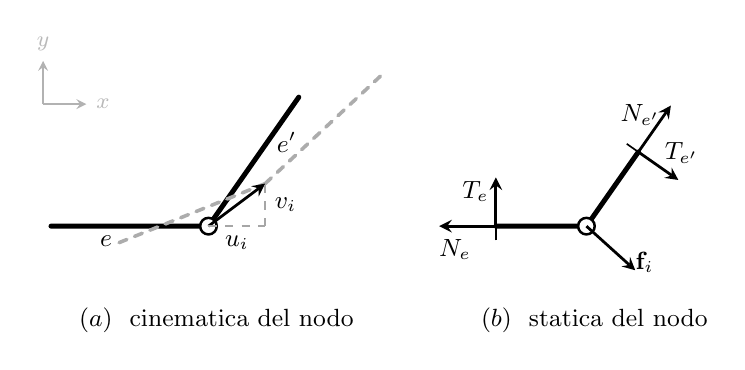
\begin{tikzpicture}[
			trave/.style={line width=1.8pt, line cap=round, line join=round, black},
			ghost/.style={line width=1.3pt, dashed, line cap=round, line join=round, gray!65},
			forza/.style={->, >=stealth, line width=1.0pt, black},
			momento/.style={->, >=stealth, line width=0.9pt, black},
			guida/.style={line width=0.55pt, dashed, gray!70},
			taglio/.style={line width=0.6pt, black},
			asse/.style={->, >=stealth, line width=0.6pt, gray!60},
			cerniera/.style={circle, draw=black, fill=white, line width=0.9pt, inner sep=0pt, minimum size=6pt},
			lab/.style={font=\small},
			labg/.style={font=\footnotesize, gray!55},
			]
			
			\def\Le{2.0}      % trave e (orizzontale, a sinistra del nodo)
			\def\Lep{2.0}     % trave e'
			\def\ang{55}      % inclinazione di e'  (angolo incluso ~125°)
			\def\SEP{4.8}     % separazione tra i pannelli
			
			%%═══ PANNELLO (a) — cinematica del nodo ══════════════════════════
			\begin{scope}
				% configurazione indeformata
				\draw[trave] (-\Le,0) -- (0,0) -- ({\Lep*cos(\ang)},{\Lep*sin(\ang)});
				% traslazione CONDIVISA, rotazioni INDIPENDENTI
				\def\du{0.72}\def\dv{0.54}
				\def\rote{22}     % rotazione trave e
				\def\rotep{-12}   % rotazione trave e' (diversa: la cerniera lascia libera la rotazione relativa)
				% configurazione spostata: nodo traslato, ogni trave ruotata per conto proprio attorno al nodo
				\begin{scope}[shift={(\du,\dv)}]
					\draw[ghost, rotate=\rote]  (-\Le,0) -- (0,0);
					\draw[ghost, rotate=\rotep] (0,0) -- ({\Lep*cos(\ang)},{\Lep*sin(\ang)});
				\end{scope}
				% cerniera al nodo (configurazione di riferimento)
				\node[cerniera] at (0,0) {};
				% spostamento nodale condiviso e componenti nel riferimento globale
				\draw[forza] (0,0) -- (\du,\dv);
				\draw[guida] (0,0) -- (\du,0);
				\draw[guida] (\du,0) -- (\du,\dv);
				\node[lab, below] at ({\du/2},0) {$u_i$};
				\node[lab, right] at (\du,{\dv/2}) {$v_i$};
				% rotazioni indipendenti — archi simbolici al nodo traslato  [POSIZIONI DA RIFINIRE]
				%				\draw[momento, line width=1.0pt] ({\du+0.42*cos(150)},{\dv+0.42*sin(150)}) arc (150:205:0.42);
				%				\node[lab] at ({\du-0.42},{\dv+0.50}) {$\vartheta_e$};
				%				\draw[momento, line width=1.0pt] ({\du+0.46*cos(82)},{\dv+0.46*sin(82)}) arc (82:37:0.46);
				%				\node[lab] at ({\du+0.42},{\dv+0.68}) {$\vartheta_{e'}$};
				% etichette travi
				\node[lab, below] at (-1.30,0) {$e$};
				\node[lab, right] at ({1.30*cos(\ang)},{1.30*sin(\ang)}) {$e'$};
				% assi globali
				\begin{scope}[shift={(-\Le-0.10,1.55)}]
					\draw[asse] (0,0) -- (0.55,0) node[labg, right] {$x$};
					\draw[asse] (0,0) -- (0,0.55) node[labg, above] {$y$};
				\end{scope}
				\node[lab] at (0.10,-1.20) {$(a)$ \ cinematica del nodo};
			\end{scope}
			
			%%═══ PANNELLO (b) — statica del nodo (corpo libero) ══════════════
			\begin{scope}[xshift=\SEP cm]
				\def\dc{1.15}   % posizione del taglio lungo ciascuna trave
				% tronconi isolati delle due travi
				\draw[trave] (-\dc,0) -- (0,0) -- ({\dc*cos(\ang)},{\dc*sin(\ang)});
				% cerniera al nodo (perno)
				\node[cerniera] at (0,0) {};
				
				% ---- estremità della trave e (taglio a sinistra): trasmette N, T; M = 0 ----
				\draw[taglio] (-\dc,-0.18) -- (-\dc,0.18);            % sezione
				\draw[forza]  (-\dc,0) -- (-\dc-0.72,0);              % N_e (trazione, uscente)
				\node[lab] at (-\dc-0.52,-0.30) {$N_e$};
				\draw[forza]  (-\dc,0) -- (-\dc,0.62);                % T_e (trasversale, verso l'alto)
				\node[lab] at (-\dc-0.26,0.44) {$T_e$};
				
				% ---- estremità della trave e' (taglio in alto a destra): trasmette N, T; M = 0 ----
				\begin{scope}[shift={({\dc*cos(\ang)},{\dc*sin(\ang)})}, rotate=\ang]
					\draw[taglio] (0,-0.18) -- (0,0.18);              % sezione
					\draw[forza]  (0,0) -- (0.72,0);                  % N_{e'} (trazione, uscente)
					\node[lab] at (0.40,0.25) {$N_{e'}$};
					\draw[forza]  (0,0) -- (0,-0.62);                 % T_{e'} (invertito)
					\node[lab] at (0.30,-0.46) {$T_{e'}$};
				\end{scope}
				
				% carico nodale esterno (eventuale): sola forza f_i
				% (una coppia concentrata non è trasmessa dalla cerniera: cfr. nota nel testo)
				\draw[forza] (0,0) -- (0.62,-0.56);
				\node[lab, right] at (0.50,-0.46) {$\mathbf{f}_i$};
				
				\node[lab] at (0.10,-1.20) {$(b)$ \ statica del nodo};
			\end{scope}
			
		\end{tikzpicture}
	}%
	\caption{Cerniera interna tra due travi, $e$ ed $e'$. A sinistra:
		cinematica del nodo --- le traslazioni $(u_i, v_i)$ nel
		riferimento globale sono condivise da entrambe le travi,
		mentre le rotazioni $\vartheta_e$ e $\vartheta_{e'}$ restano
		indipendenti: l'angolo tra le travi non si conserva.
		A destra: statica del nodo isolato come corpo libero ---
		ciascuna trave trasmette le sole caratteristiche di forza
		$N$ e $T$ nel rispettivo sistema locale, mentre il momento
		non è trasmesso ($M = 0$ su ciascun elemento); con
		l'eventuale carico nodale $\mathbf{f}_i$, l'equilibrio del
		nodo si riduce a $\sum\mathbf{f}=\mathbf{0}$ --- due
		equazioni scalari, una in meno del nodo rigido.}
	\label{fig:cerniera_interna}
\end{figure}
%%%%%%%%%%%%%%%%%%%%%%%%%%%%%%%%%%%%%%%%%%%




%%%%%%%%%%%%%%%%%%%%%%%%%%%%%%%%%%%%%%%%%%%
\begin{figure}[htbp]
	\centering
	%\includegraphics[scale=0.75]{cerniera_interna.pdf}
	\caption{Cerniera interna tra due travi. A sinistra:
		schema cinematico --- le traslazioni $u$, $v$
		sono uguali, le rotazioni $\vartheta_e$,
		$\vartheta_{e'}$ sono indipendenti.
		A destra: schema statico --- la cerniera
		trasmette $N$ e $T$ ma impone $M = 0$ su
		ciascun elemento; la reazione interna
		$\mathbf{f}_C^\mathscr{v}$ con le sue due
		componenti è indicata esplicitamente.}
	\label{fig:cerniera_interna}
\end{figure}
%%%%%%%%%%%%%%%%%%%%%%%%%%%%%%%%%%%%%%%%%%%


%............................................................................................................................
\subsection{Carrello interno}
\label{subsec:carrello_interno}
%............................................................................................................................

Il \emph{carrello interno}\index{carrello!interno} (detto anche giunzione
scorrevole o cerniera scorrevole) consente spostamenti
relativi in una direzione assegnata oltre alla
rotazione relativa. Indicata con $\bm{a}$ la direzione
vincolata (normale alla direzione di scorrimento),
la condizione di congruenza nel nodo $i$ è:
\begin{equation}\label{eq:cong_carrello_int}
	\mathbf{u}_e(i) \cdot \mathbf{a} = u_{i,a}, \qquad 
	\forall\, e \in \mathcal{E}_i,
\end{equation}
dove $u_{i,a}$ è la componente dello spostamento
nodale nella direzione $\mathbf{a}$, condivisa da tutte
le $e_i$ travi convergenti, mentre la componente
ortogonale a $\mathbf{a}$ e le rotazioni $\vartheta_e(i)$
sono libere e in generale diverse per ciascuna trave.

\paragraph{Lettura cinematica.}
Il carrello interno impone la continuità della sola
\emph{componente di spostamento nella direzione vincolata}.
La sua molteplicità è $m_i = 1$.

\paragraph{Lettura statica.}
Il carrello interno trasmette la sola componente
di \emph{forza nella direzione vincolata}: se $\bm{a}$
è la direzione ortogonale all'asse di scorrimento,
soltanto la componente di forza in quella direzione
è trasmessa tra i due elementi. Le forze nella direzione
di scorrimento e il momento flettente sono entrambi nulli
agli estremi degli elementi nel nodo.

\begin{oss}
	I tre tipi di connessione --- nodo rigido, cerniera,
	carrello --- formano una gerarchia di molteplicità
	decrescente: $m_i = 3,\, 2,\, 1$. Ciascuno si ottiene
	dal precedente rilasciando progressivamente un grado
	di libertà (prima la rotazione, poi una traslazione).
	Sul versante statico, il rilascio di un grado di libertà
	cinematico corrisponde all'annullamento della corrispondente
	caratteristica della sollecitazione nel nodo.
	Questa dualità è la manifestazione locale di
	$\bm{B} = \bm{A}^{\top}$: ogni riga in meno in $\bm{A}$
	(un vincolo in meno) corrisponde a una colonna in meno
	in $\bm{B}$ (una caratteristica trasmessa in meno).
\end{oss}


%............................................................................................................................
\subsection{Formula generale della molteplicità per nodi
	con $e_i$ travi convergenti}
\label{subsec:molt_generale}
%............................................................................................................................

Quando in un nodo $i$ convergono $e_i \geq 2$ travi,
la molteplicità del vincolo interno si calcola
moltiplicando la molteplicità intrinseca del tipo
di connessione per il numero di relazioni di uguaglianza
da imporre. La prima trave è assunta come riferimento:
per ognuna delle $e_i - 1$ travi rimanenti si impongono
le condizioni di congruenza rispetto alla prima.
Ne risulta la formula:
\begin{equation}\label{eq:molt_nodo}
	m_i =
	\begin{cases}
		3\,(e_i - 1) & \text{nodo rigido,} \\[4pt]
		2\,(e_i - 1) & \text{cerniera interna,} \\[4pt]
		1\,(e_i - 1) & \text{carrello interno (direzione } \bm{a}\text{).}
	\end{cases}
\end{equation}

\begin{oss}
	La formula~\EQUref{eq:molt_nodo} mostra che la
	molteplicità cresce \emph{linearmente} con il numero
	di travi convergenti. Nodi di diramazione (con $e_i \geq 3$)
	contribuiscono quindi al vincolo in modo molto più
	significativo dei semplici nodi di continuità ($e_i = 2$).
	Questo vale in modo particolarmente marcato per i nodi
	rigidi dei telai, dove $m_i = 3(e_i - 1)$ può
	risultare elevato già con tre o quattro travi convergenti.
\end{oss}

\begin{oss}[Nodi misti]
	In alcuni nodi, non tutte le travi convergenti sono
	collegate con la stessa tipologia: ad esempio, una trave
	può essere saldata rigidamente mentre un'altra è
	connessa con cerniera. In questi casi la
	formula~\EQUref{eq:molt_nodo} non si applica
	direttamente: occorre contare separatamente le condizioni
	di congruenza per ciascuna coppia, verificando le
	relazioni di uguaglianza effettivamente imposte.
	La sezione~\EQUref{eq:cong_nodo_rigido}--\EQUref{eq:cong_carrello_int}
	fornisce le equazioni di base per ogni coppia; la loro
	combinazione per nodi misti non presenta difficoltà
	concettuali ma richiede attenzione nella contabilizzazione.
\end{oss}

La \TABref{tab:connessioni} riassume le tre tipologie
di connessione con le relative molteplicità per $e_i = 2$
e le caratteristiche trasmesse.

%%%%%%%%%%%%%%%%%%%%%%%%%%%%%%%%%%%%%%%%%%%
\begin{table}[htbp]
	\centering
	\renewcommand{\arraystretch}{1.6}
	\begin{tabular}{lcccccc}
		\toprule
		\textbf{Connessione} & $m_i$ & \textbf{Vincolato} &
		\textbf{Libero} & $N$ & $T$ & $M$ \\
		\midrule
		Nodo rigido      & 3 & $u,\,v,\,\vartheta$ & --- &
		\checkmark & \checkmark & \checkmark \\
		Cerniera interna & 2 & $u,\,v$ & $\vartheta_e$ &
		\checkmark & \checkmark & $0$ \\
		Carrello interno (trasversale) & 1 & $v_e$ & $\vartheta_e$, $w_e$ &
		$0$ & \checkmark & $0$ \\
		Carrello interno (longitudinale) & 1 & $w_e$ & $\vartheta_e$, $v_e$ &
		\checkmark & $0$ & $0$ \\
		\bottomrule
	\end{tabular}
	\caption{Tipologie di connessione interna per $e_i = 2$
		travi convergenti. Colonna $m_i$: molteplicità
		del vincolo interno. Colonne \emph{Vincolato}
		e \emph{Libero}: componenti di spostamento
		vincolate --- espresse nel riferimento globale per il nodo rigido e la cerniera,
		condivise da tutte le travi convergenti --- e
		libere --- rotazioni $\vartheta_e$ indipendenti
		per ciascuna trave. Colonne $N$, $T$, $M$:
		caratteristiche della sollecitazione trasmesse
		(\checkmark) o nulle ($0$) nel nodo per ogni
		elemento convergente, con riferimento al sistema
		locale di ciascuna trave; si veda il testo.}
	\label{tab:connessioni}
\end{table}
%%%%%%%%%%%%%%%%%%%%%%%%%%%%%%%%%%%%%%%%%%%

%----------------------------------------------------------------------------------------------------------------------------
\section{Procedura operativa per sistemi di travi}
\label{sec:procedura_operativa}
%----------------------------------------------------------------------------------------------------------------------------

Le strategie di analisi sviluppate nel
\CAPref{cap:classificazione_sol_SCR} per i sistemi di
corpi rigidi si applicano direttamente ai sistemi di
travi. Il presente paragrafo ne declina la versione
specializzata al contesto delle travi, identificando
i passi che nella pratica precedono il calcolo esplicito.

La procedura si articola in cinque passi, che è utile
seguire nell'ordine indicato perché ciascuno condiziona
i successivi.

\medskip
\noindent\textbf{Passo 1 — Identificazione degli elementi
	e delle connessioni.}
Si individuano le $n_e$ travi del sistema, numerandole
sistematicamente, e per ciascun nodo si identifica:
il tipo di connessione (rigido, cerniera, carrello),
il numero $e_i$ di travi convergenti e la presenza
di eventuali vincoli esterni. Questa fase è topologica:
non richiede calcoli, ma una lettura attenta dello
schema strutturale.

\medskip
\noindent\textbf{Passo 2 — Conteggio e classificazione
	preliminare.}
Si calcolano:
\begin{equation}\label{eq:conteggio_travi}
	n = 3n_e, \qquad
	m = m_{\text{est}} + m_{\text{int}}, \qquad
	\nu = n - m = 3n_e - m,
\end{equation}
dove $m_{\text{est}}$ si ricava dalle molteplicità dei
vincoli esterni (\CAPref{cap:vincoli_CR}) e
$m_{\text{int}}$ dalla \EQUref{eq:molt_nodo}.
Il valore di $\nu$ fornisce la classificazione
\emph{nominale}: $\nu > 0$ sistema certamente labile,
$\nu = 0$ caso nominalmente isostatico, $\nu < 0$
sistema certamente iperstatico. Come già discusso nel
\CAPref{cap:classificazione_SCR}, il conteggio è
condizione necessaria ma non sufficiente: la
classificazione effettiva dipende dal rango della
matrice dei vincoli, che può essere deficiente in
presenza di disposizioni geometriche degeneri.

\medskip
\noindent\textbf{Passo 3 — Separazione esterno/interno.}
Si analizza il comportamento esterno trattando il sistema
come un unico corpo rigido e considerando i soli vincoli
al suolo: si verifica se i vincoli esterni bloccano
tutti i moti rigidi d'insieme ($g_\ell^{\text{est}} = 0$),
se ne lasciano liberi alcuni ($g_\ell^{\text{est}} > 0$,
labilità esterna)\index{labilita@labilità!esterna} o se sono sovrabbondanti
($g_{\mathscr{i}}^{\text{est}} > 0$, iperstaticità
esterna)\index{iperstaticita@iperstaticità!esterna}. Si analizza poi il comportamento interno,
verificando se le connessioni tra le travi introducono
meccanismi interni o vincoli ridondanti interni,
indipendentemente dai vincoli al suolo.

\medskip
\noindent\textbf{Passo 4 — Verifica delle condizioni
	geometriche.}
Si controllano le condizioni geometriche che garantiscono
la non degenerazione del sistema: parallelismo o
concorrenza degli assi dei vincoli per i sistemi a
corpo singolo, allineamento dei centri di istantanea
rotazione per sistemi a più corpi. Questo passo è
cruciale perché un sistema nominalmente isostatico
($\nu = 0$) può essere in realtà degenere se i vincoli
sono disposti in modo particolare, come discusso nel
catalogo delle sottostrutture del
\CAPref{cap:classificazione_SCR}.

\medskip
\noindent\textbf{Passo 5 — Impostazione dell'analisi.}
Una volta classificato il sistema, si sceglie la
strategia di soluzione appropriata:
\begin{itemize}[noitemsep]
	\item per i sistemi \emph{isostatici} si procede
	con il metodo dei corpi liberi per il problema
	statico e con il metodo grafo-analitico per
	quello cinematico, sfruttando la gerarchia
	strutturale quando presente
	(\CAPref{cap:classificazione_sol_SCR});
	\item per i sistemi \emph{iperstatici} si
	individua un sistema principale isostatico,
	si parametrizza la soluzione nelle incognite
	iperstatiche $\chi_j$\index{iperstaticita@iperstaticità!incognita iperstatica} e si rimanda la loro
	determinazione ai metodi del Vol.~II;
	\item per i sistemi \emph{labili} si identificano
	i meccanismi e le eventuali condizioni di
	compatibilità sui carichi.
\end{itemize}

\begin{oss}
	I passi 1--4 costituiscono l'\emph{analisi
		qualitativa preliminare} del sistema, analoga
	a quella introdotta per la trave singola nel
	\CAPref{cap:Diagrammi_CS}. Come lì, essa non è
	un lusso ma una necessità: identificare il tipo
	di sistema prima di impostare le equazioni evita
	di cercare soluzioni che non esistono o di
	trascurare gradi di libertà che rendono la
	soluzione non unica.
\end{oss}


%------------------------------------------------------------
\section{Catalogo delle tipologie strutturali}
\label{sec:catalogo}
%------------------------------------------------------------

Le tipologie strutturali che seguono costituiscono il
vocabolario fondamentale degli assemblaggi di travi piane.
Esse si organizzano naturalmente in due famiglie,
distinte dalla natura delle connessioni tra le travi.

I \emph{sistemi a connessioni eterogenee}\index{connessione!eterogenea|textbf} ammettono
connessioni di tipo diverso --- nodi rigidi, cerniere
interne, carrelli interni, appoggi semplici --- all'interno
dello stesso sistema. La formula di classificazione
$\nu = 3n_e - m$ si applica senza modifiche, con $m$
calcolato sommando le molteplicità di ciascuna connessione
secondo la \EQUref{eq:molt_nodo}. L'analisi procede con
la prima lettura topologica\index{lettura topologica|textbf} --- travi come corpi rigidi,
connessioni come vincoli --- e si risolve con il metodo
dei corpi liberi già sviluppato per la trave singola.
Le configurazioni isostatiche di questa famiglia ---
travi di Gerber\index{trave!di Gerber}, sistemi a tre cerniere e assemblaggi
vari --- sono trattate in dettaglio nel
\CAPref{cap:sistemi_conn_eterogenee}; le configurazioni iperstatiche
(travi continue)\index{trave!continua} richiedono i metodi del Vol.~II.

I \emph{sistemi a connessioni omogenee}\index{connessione!omogenea|textbf} si dividono
in due tipologie estreme: i \emph{sistemi reticolari}\index{sistema reticolare},
in cui tutte le connessioni sono cerniere ($m_i = 1$),
e i \emph{telai}\index{telaio}, in cui tutte le connessioni sono
nodi rigidi ($m_i = 3$). Per entrambi, l'omogeneità
delle connessioni rende possibile una \emph{seconda
	lettura topologica}\index{lettura topologica!seconda} in cui i nodi diventano i
protagonisti e le travi i vincoli: questa prospettiva
conduce a equazioni cinematiche e statiche di struttura
particolarmente trasparente, esplicitate nei
\CAPref{cap:reticolari} e~\CAPref{cap:telai_piani}.

I sistemi reticolari ammettono configurazioni
isostatiche paradigmatiche --- analizzabili con il
solo equilibrio e sviluppate nel \CAPref{cap:reticolari}
--- ma anche configurazioni iperstatiche, quando i
vincoli esterni sono sovrabbondanti oppure il numero
di aste supera il minimo necessario per l'isostaticità
interna, o entrambe le cose. I telai sono invece
intrinsecamente iperstatici nella configurazione
standard con maglie chiuse, indipendentemente dai
vincoli esterni.

In questo volume si trattano le configurazioni
isostatiche dei sistemi a connessioni eterogenee e
dei sistemi reticolari, perché in entrambi i casi
la procedura di analisi --- classificazione,
cinematica e determinazione delle caratteristiche
della sollecitazione --- è completa con i soli
strumenti dell'equilibrio. Per tutte le configurazioni
iperstatiche --- sistemi eterogenei, reticolari o
telai, con sovradeterminazione esterna o interna
o entrambe --- le equazioni di equilibrio non sono
sufficienti: il numero di incognite statiche supera
il numero di equazioni disponibili. Le incognite
iperstatiche si determinano imponendo le condizioni
di compatibilità cinematica, che coinvolgono
necessariamente il legame costitutivo tra sforzi
e deformazioni. È questo legame che introduce le
proprietà del materiale e della sezione trasversale
nell'analisi strutturale, e che richiede gli
strumenti sviluppati nel Vol.~II.

Il catalogo delle tipologie strutturali si articola
nei capitoli che seguono, organizzati secondo la
natura delle connessioni.

I \emph{sistemi a connessioni eterogenee} ---
assemblaggi ramificati con nodi rigidi, sistemi a tre
cerniere, travi continue e travi di Gerber 
--- sono trattati nel \CAPref{cap:sistemi_conn_eterogenee}.
Per queste tipologie la prima lettura topologica
è lo strumento naturale di analisi: le connessioni
di tipo diverso determinano una gerarchia
strutturale che consente la risoluzione in cascata
e il tracciamento delle caratteristiche della
sollecitazione sull'intera struttura. La varietà
degli schemi trattati mostra come la stessa
procedura operativa si applichi a geometrie e
topologie molto diverse, dal sistema ramificato con nodi
rigidi al sistema lineare della
trave di Gerber.

I \emph{sistemi reticolari} --- connessioni
esclusivamente a cerniera --- sono trattati nel
\CAPref{cap:reticolari}. La seconda lettura
topologica, in cui i nodi sono i protagonisti
e le aste i vincoli, conduce alla formula di
Müller-Breslau e ai metodi operativi --- metodo
dei nodi e metodo delle sezioni di Ritter ---
per la determinazione degli sforzi normali nelle
travature isostatiche.

I \emph{telai} --- connessioni esclusivamente
rigide con maglie chiuse --- sono trattati nel
\CAPref{cap:telai_piani}. La seconda lettura topologica
conduce alle equazioni di compatibilità nodale e
alle equazioni di equilibrio nodale con $N$, $T$,
$M$ come incognite. I telai sono intrinsecamente
iperstatici e la loro analisi completa richiede
le relazioni costitutive sviluppate nel Vol.~II;
il \CAPref{cap:telai_piani} ne costruisce i fondamenti
topologici e la struttura formale.

